\documentclass{beamer}
\usepackage{graphicx}
\usepackage{apacite}
\usepackage{multimedia}

% turn off controls at bottom of slide
\setbeamertemplate{navigation symbols}{}

% set theme
\mode<presentation>{\usetheme{Warsaw}}

\title{Spiral Galaxies}
\author{Charlie Redmon}
\date{12 April 2013}

\begin{document}

\begin{frame}
\titlepage
\end{frame}

\section{Overview}

\begin{frame}[t]
\frametitle{Overview}

	\begin{itemize}
	\item<2->What are spiral galaxies?
	\item<3->Structure
	\item<4->Famous spiral galaxies
	\item<5->Galaxy formation
	\end{itemize}
\end{frame}

\section{What are spiral galaxies}

\begin{frame}[t]
\frametitle{What are spiral galaxies?}
	\begin{itemize}
	\item<2->A type of elliptical galaxy
	\item<3->Appearance: flat, rotating disk with interior 'bulge'; spiral arms extending outward from center
	\item<4->Hubble's classification:
		\begin{enumerate}
		\item<5->Binary division: barred and non-barred
		\item<6->Ternary division: (a) tightly-wound, (b) less-tightly-wound, (c) loosely-wound
		\end{enumerate}
	\item<7->Ex: Sc, SBa, Sb
	\end{itemize}
\end{frame}



\begin{frame}
\frametitle{Hubble Sequence}
\begin{figure}
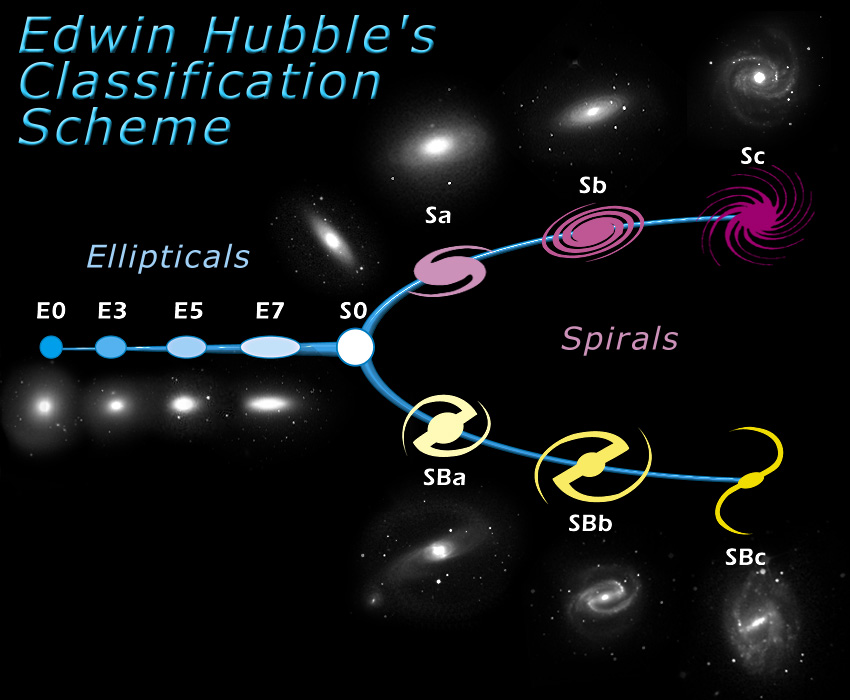
\includegraphics[width=110mm, height=60mm]{HubbleTuningFork.jpg}
\caption{Wikimedia Commons; NASA/ESA, 1999}
\end{figure}
\end{frame}

\section{Structure}

\begin{frame}[t]
\frametitle{Structure}
	\begin{itemize}
	\item<2->Spiral arms of three major types:
		\begin{enumerate}
		\item<3->Grand-design (2)
		\item<4->Multiple-arm(3+)
		\item<5->Flocculent (no well-defined spirals)
		\end{enumerate}
	\end{itemize}
\end{frame}

\begin{frame}
\frametitle{Grand-design}
\begin{figure}
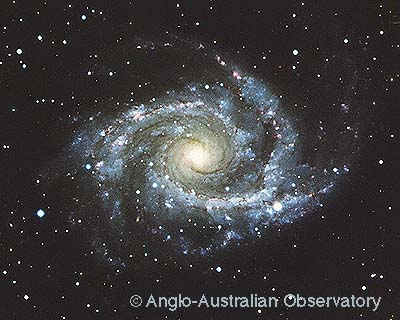
\includegraphics[width=90mm, height=65mm]{grand_design.jpg}
\end{figure}
\end{frame}

\begin{frame}
\frametitle{Flocculent}
\begin{figure}
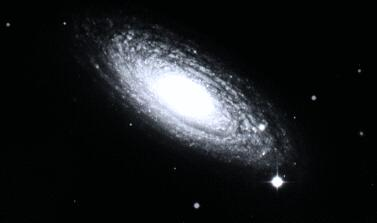
\includegraphics[width=90mm, height=65mm]{flocculent.jpg}
\end{figure}
\end{frame}

\begin{frame}[t]
\frametitle{Structure}
	\begin{itemize}
	\item<1->Spiral arms of three major types:
		\begin{enumerate}
		\item<1->Grand-design (2)
		\item<1->Multiple-arm(3+)
		\item<1->Flocculent (no well-defined spirals)
		\end{enumerate}
	\item<2->Not `solid-body' rotation curves \cite{mihos2011}
	\end{itemize}

\begin{columns}
  \begin{column}{0.5\textwidth}
    \begin{itemize}
        \item<3->Spiral at zero position
	\bigskip
	\bigskip
	\bigskip
        \item<5->Spiral at final position
    \end{itemize}
  \end{column}

  \begin{column}{0.5\textwidth}
     \begin{itemize}
        	\item[]<4-> \includegraphics[width=25mm, height=20mm]{spiral_start.png}
	\item[]<6-> \includegraphics[width=25mm, height=20mm]{spiral_finish.png}
     \end{itemize}
  \end{column}
\end{columns}
\end{frame}

\section{Famous spiral galaxies}

\begin{frame}[t]
\frametitle{Famous spiral galaxies}
\begin{center}
\begin{tabular}{|l l l l|} \hline	
Name		&	Designation	&	Classification	&	App. Mag.  			\\ \hline
Milky Way		&	N/A 			&	SBc			&	N/A 				\\
Andromeda	&	M31			&	SA(s)b  		&	4.36				\\
Pinwheel		& 	M101		&	SAB(rs)cd		& 	8.3				\\
Whirlpool		&	M51			&	SA(s)bc pec	&	9.0				\\
Sombrero 		& 	M104		& 	SA(s)a 		&	9.0				\\			 
Black Eye		&	M64			&	(R)SA(rs)ab	&	9.4				\\ \hline
\end{tabular}
\end{center}
\end{frame}

\begin{frame}[t]
\frametitle{Calculating apparent magnitude}
\begin{equation}
m_{x}-m_{x,0} = -2.5 \log_{10}\left ( \frac{F_{x}}{F_{x,0}} \right )
\end{equation}
\begin{itemize}
	\item<2->$m_x$ = apparent magnitude in the band $x$
	\item<3->$m_{x,0}$ = reference magnitude
	\item<4->$F_x$ = observed flux in band $x$
	\item<5->$F_{x,0}$ = reference flux
\end{itemize}
\end{frame}


\begin{frame}
\frametitle{The Milky Way}
\begin{figure}
\includegraphics[width=100mm, height=50mm]{paranal_milky.jpg}
\caption{European Southern Observatory: Paranal, Chile}
\nocite{eso2013}
\end{figure}
\end{frame}

\begin{frame}
\frametitle{The Andromeda Galaxy (M31)}
\begin{figure}
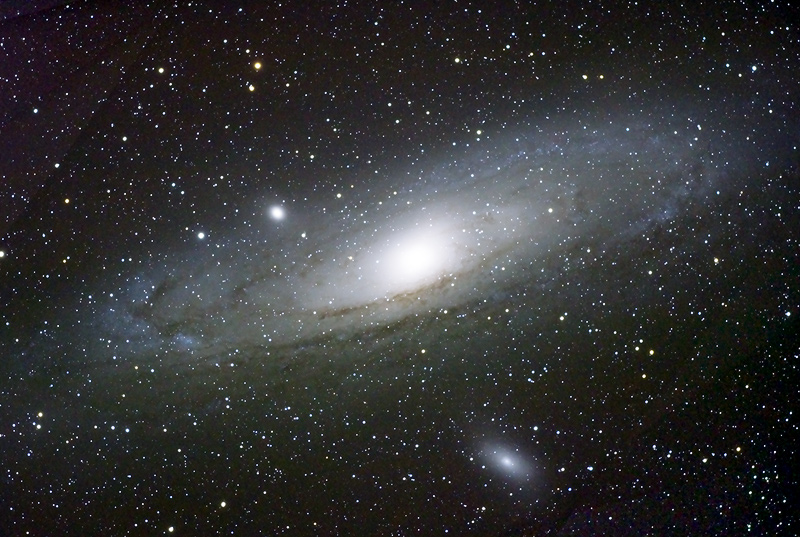
\includegraphics[width=100mm, height=60mm]{m31.jpg}
\nocite{nasa2010}
\end{figure}
\end{frame}

\begin{frame}
\frametitle{The Pinwheel Galaxy (M101)}
\begin{figure}
\includegraphics[width=100mm, height=60mm]{m101.jpg}
\nocite{nasa2010}
\end{figure}
\end{frame}

\begin{frame}
\frametitle{The Whirlpool Galaxy (M51)}
\begin{figure}
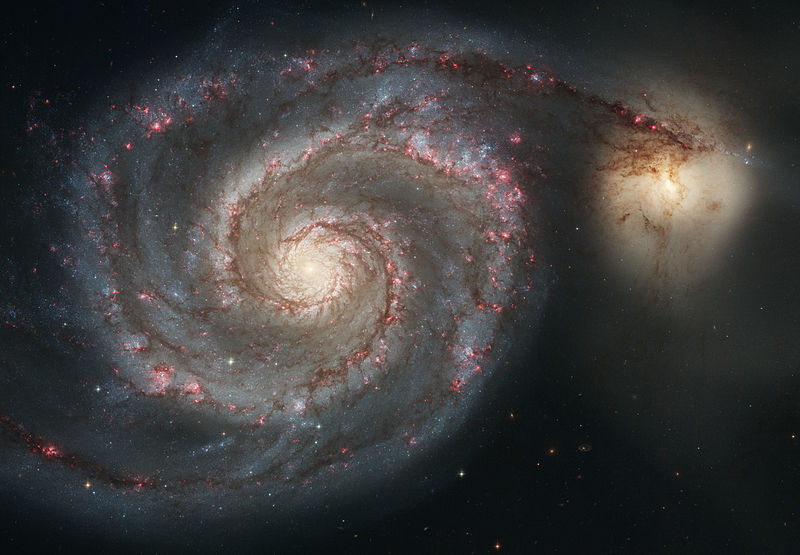
\includegraphics[width=100mm, height=60mm]{m51.jpg}
\nocite{nasa2010}
\end{figure}
\end{frame}

\begin{frame}
\frametitle{The Sombrero Galaxy (M104)}
\begin{figure}
\includegraphics[width=100mm, height=60mm]{m104.jpg}
\nocite{nasa2010}
\end{figure}
\end{frame}

\begin{frame}
\frametitle{The Black Eye Galaxy (M64)}
\begin{figure}
\includegraphics[width=100mm, height=60mm]{m64.jpg}
\nocite{nasa2010}
\end{figure}
\end{frame}


\begin{frame}
\frametitle{Galaxy formation}
\begin{center}
\movie{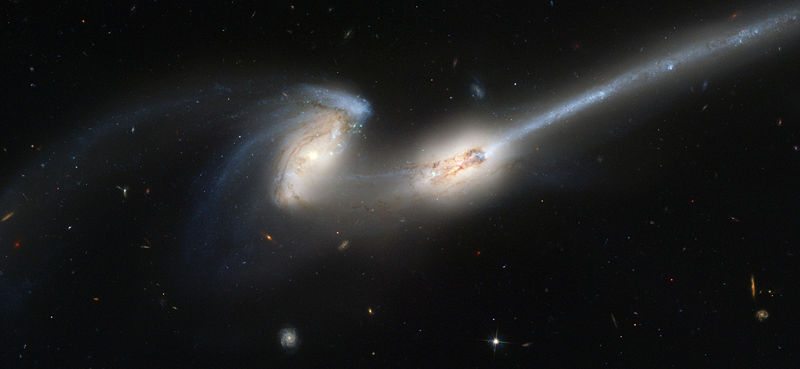
\includegraphics[width=100mm, height=60mm]{galaxy_form.jpg}}{faceon.mov}
\end{center}
\end{frame}

\section{Galaxy formation}

\begin{frame}[t]
\frametitle{References}
\bibliographystyle{apacite}
\bibliography{spiral}
\end{frame}

\end{document}